\section{Generalizirani ICP algoritam}
Eksperimantalni rezultati za generalizirajući algoritam iteracije točaka su prikazani u sljedećim tablicama i grafovima. Grafovi i tablice se odnose na podskupove točaka primjera A i B. Zbog fizičke ograničenosti računala ICP algoritam je izvršen na manjem skupu podataka. Može se zaključiti da mnogo faktora utječe na točnost estimacije lokacija. Neki odnjih su složenost okoline, brzina prikupljanja podataka, ubrzanja vozila, tip algoritma, \dots

\subsubsection{Tablica eksprimentalnih rezultata}
\begin{table}[H]
  \begin{tabular}{ |p{3cm}| |p{2cm}|p{2cm}|p{2cm}|p{2cm}| }
    \hline
    Rezultati& Primjer 1& Primjer 2&Primjer 3& Primjer 4\\
    \hline
    AMx [$m$]& 0.18427& 2.7368E-3& 1.41374E-3& 3.63932E-2\\
    AMy [$m$]&  16.3356& 1.38002E-3& 2.8428E-3& 1.32941E-2\\
    AMz [$m$]& 0.01657& 4.02492E-3& 5.811E-4& 8.78942E-4\\
    AMr [$rad$]& 1.53082E-3& 9.69565E-5& 4.95289E-5& 1.44264E-4\\
    AMp [$rad$]& 6.81777E-3& 8.68708E-5& 3.69849E-4& 2.43620E-4\\
    AMy [$rad$]& 5.63752E-2& 2.7926E-2& 1.07866E-2& 4.73278E-3\\
    \hline
    MSEx [$m^2$]& 3.9456E-2& 1.11415E-5& 3.99733E-6& 1.70555E-3\\
    MSEy [$m^2$]& 366.32160& 2.47215E-6& 1.61632E-5& 2.75735E-4\\
    MSEz [$m^2$]& 4.89075E-4& 2.15913E-5& 6.75381E-7& .98995E-7\\
    MSEr [$rad^2$]& 1.42492E-5& 1.17012E-8& 4.90623E-9& 5.0858E-8\\
    MSEp [$rad^2$]& 7.38958E-5& 1.38325E-8& 2.73577E-7& 8.0916E-8\\
    MSEy [$rad^2$]& 3.71623E-3& 1.05195E-3& 2.32704E-4& 2.94429E-5\\
    \hline
  \end{tabular}
  \caption{Usporedbe referentnih i estimiranih podataka}
  \label{res:ref_est_table}
\end{table}
\pagebreak
\subsubsection{Grafovi ekspreimentalnih rezultata}
\begin{figure}[H]
  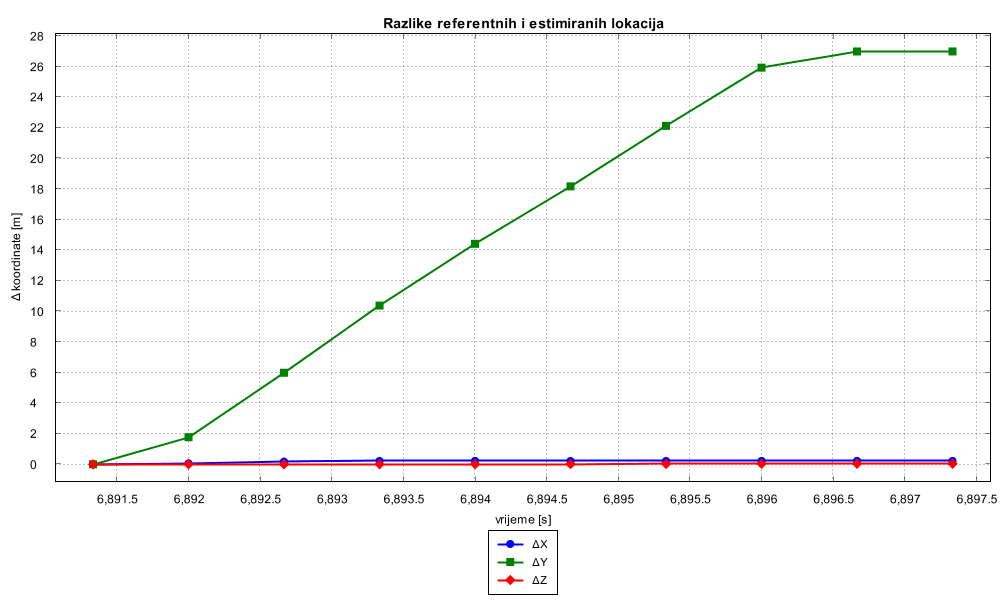
\includegraphics[scale=0.4]{images/imgs/1_zavoj_lokacije.png}
  \caption{Primjer 1 - Graf usporedbe lokacija vozila}
  \label{eval:primjer_1_lokacija}
\end{figure}
\begin{figure}[H]
  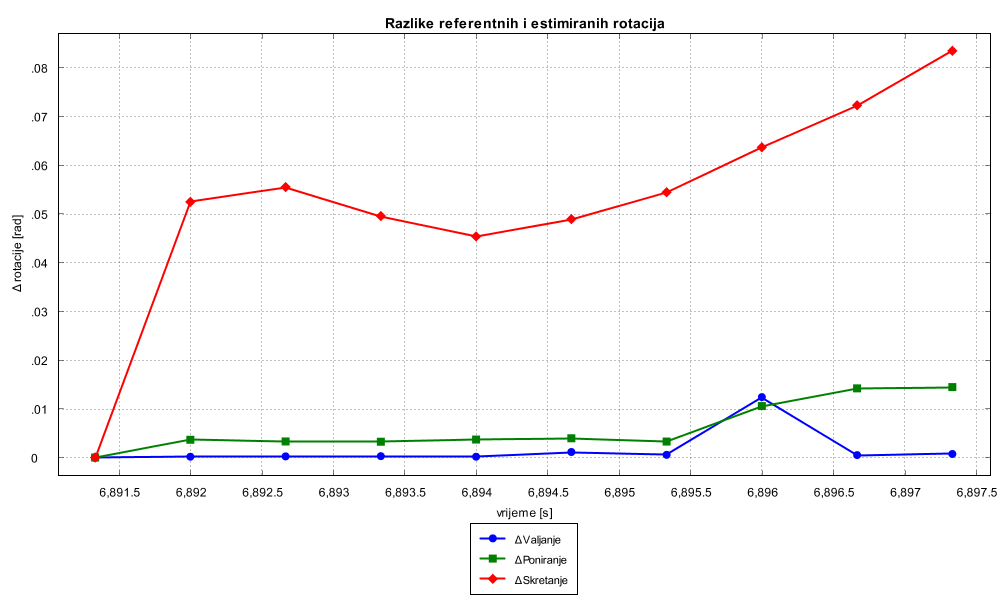
\includegraphics[scale=0.4]{images/imgs/1_zavoj_rotacije.png}
  \caption{Primjer 1 - Graf usporedbe rotacija vozila}
  \label{eval:primjer_1_rotacija}
\end{figure}
\begin{figure}[H]
  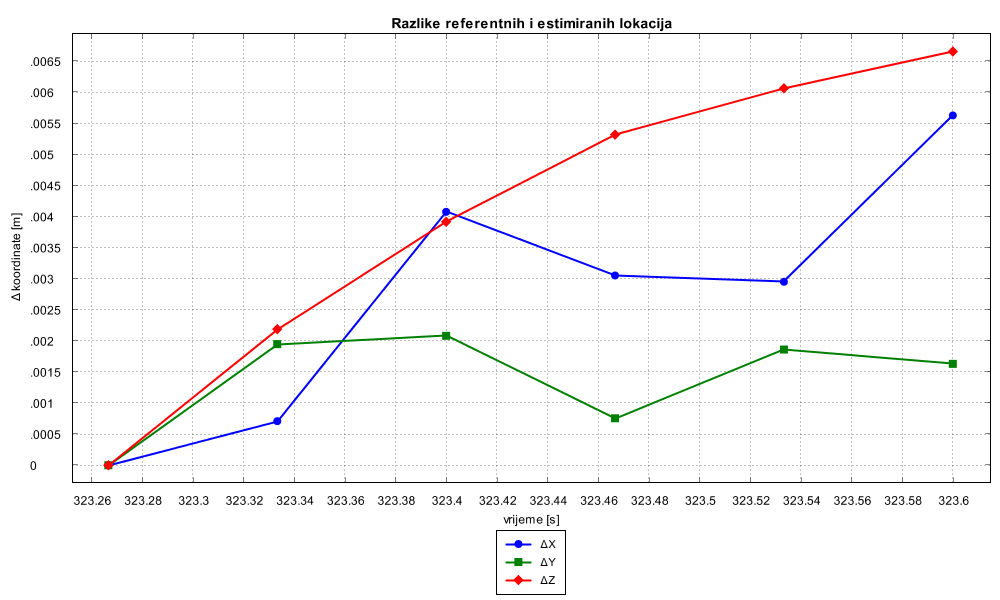
\includegraphics[scale=0.4]{images/imgs/2_ravno_lokacije.png}
  \caption{Primjer 2 - Graf usporedbe lokacija vozila}
  \label{eval:primjer_2_lokacija}
\end{figure}
\begin{figure}[H]
  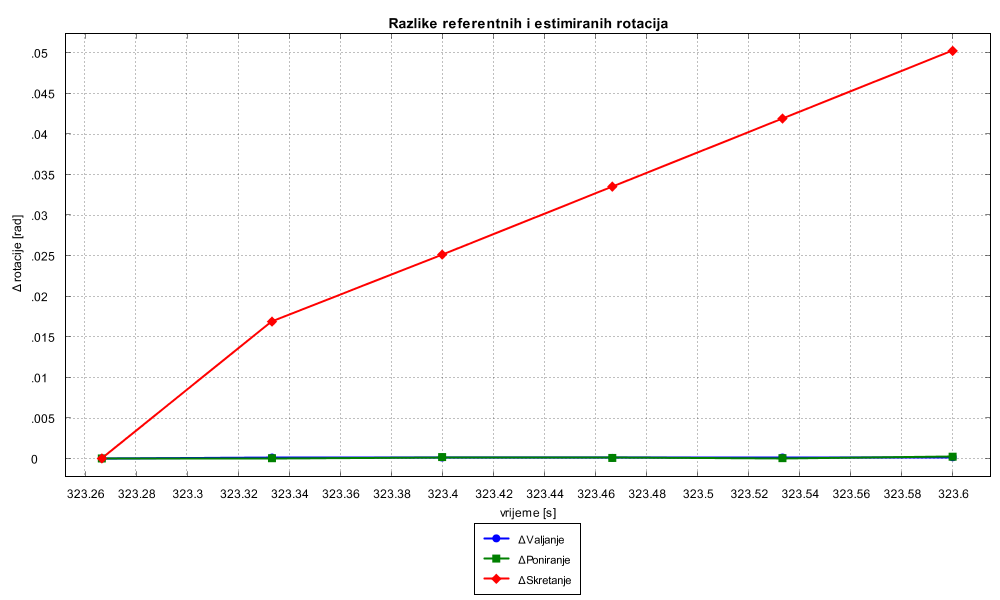
\includegraphics[scale=0.4]{images/imgs/2_ravno_rotacije.png}
  \caption{Primjer 2 - Graf usporedbe rotacija vozila}
  \label{eval:primjer_2_rotacija}
\end{figure}
\begin{figure}[H]
  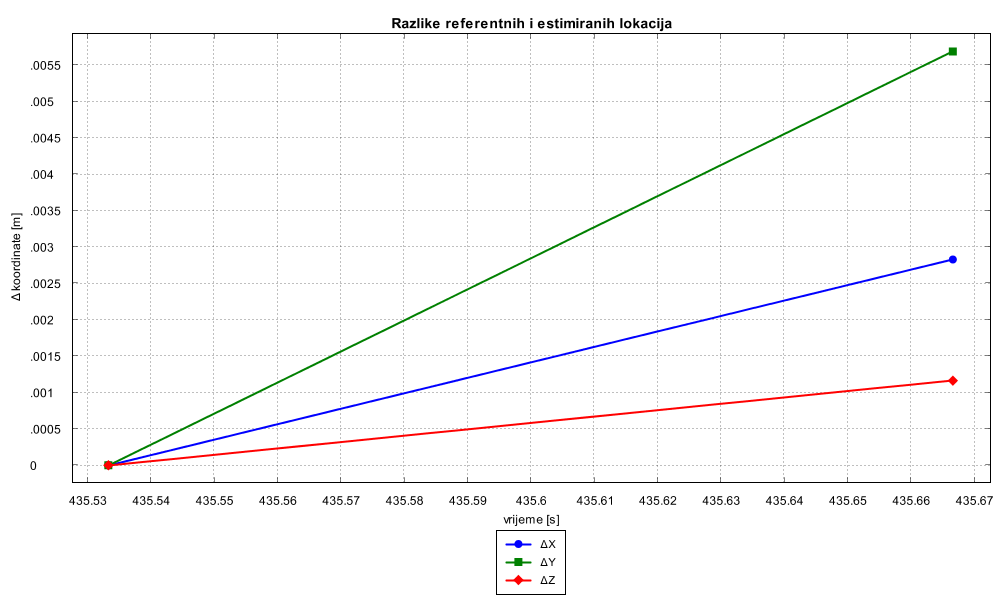
\includegraphics[scale=0.4]{images/imgs/3_ravno_lokacije.png}
  \caption{Primjer 3 - Graf usporedbe lokacija vozila}
  \label{eval:primjer_3_rotacija}
\end{figure}
\begin{figure}[H]
  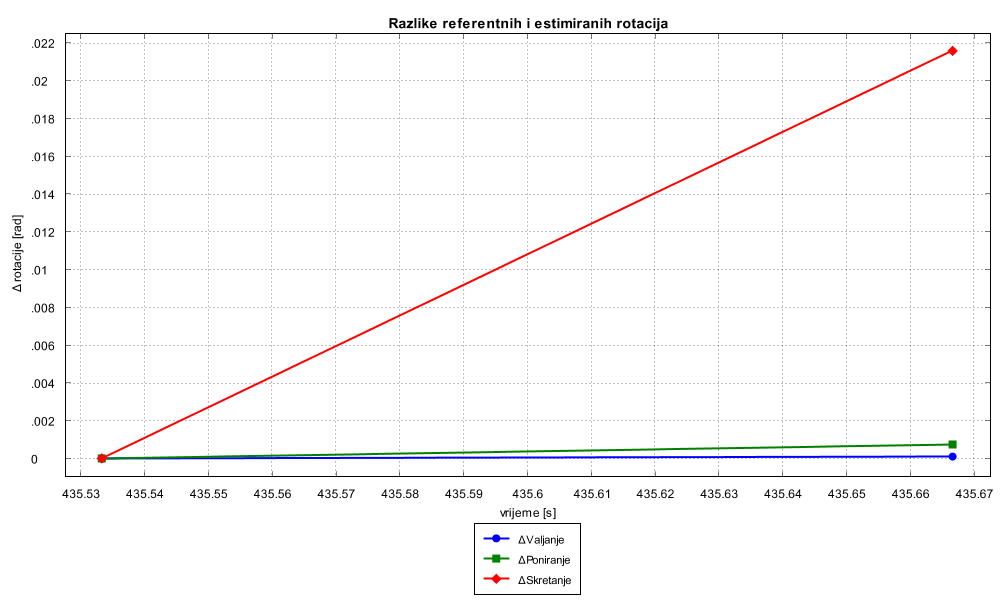
\includegraphics[scale=0.4]{images/imgs/3_ravno_rotacije.png}
  \caption{Primjer 3 - Graf usporedbe rotacija vozila}
  \label{eval:primjer_3_rotacija}
\end{figure}
\begin{figure}[H]
  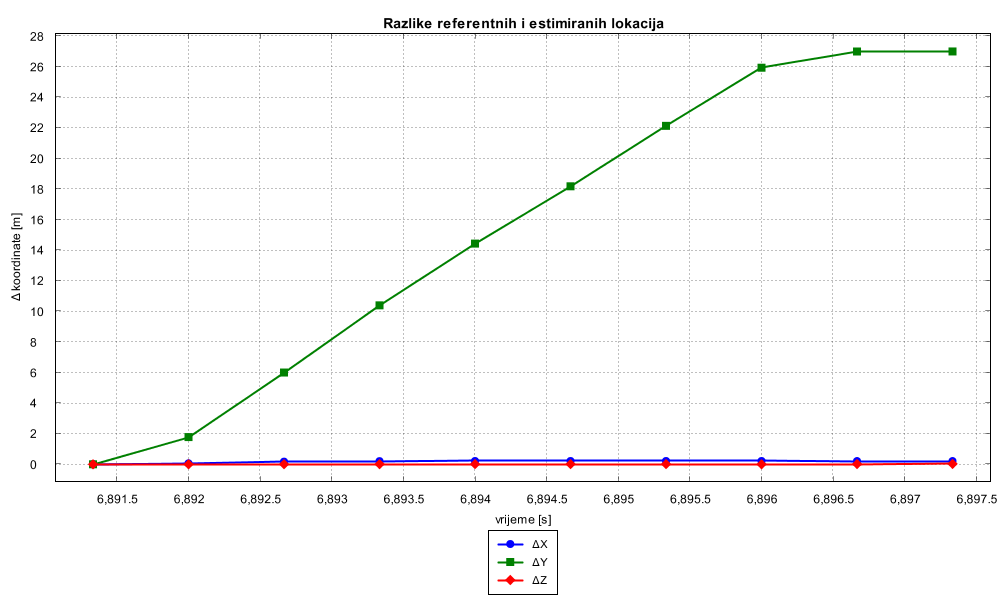
\includegraphics[scale=0.4]{images/imgs/4_zavoj_lokacije.png}
  \caption{Primjer 4 - Graf usporedbe lokacija vozila}
  \label{eval:primjer_4_rotacija}
\end{figure}
\begin{figure}[H]
  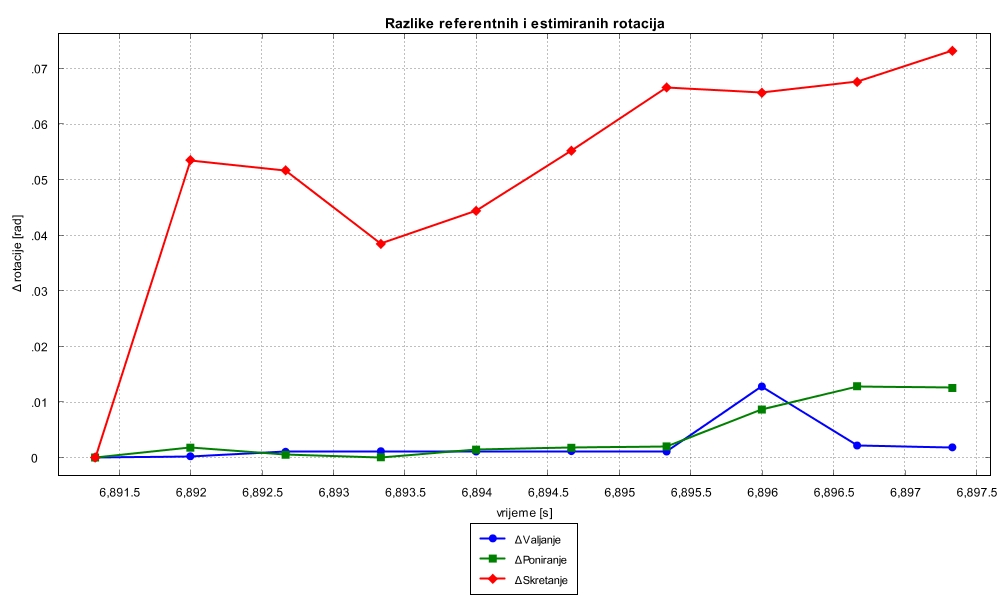
\includegraphics[scale=0.4]{images/imgs/4_zavoj_rotacije.png}
  \caption{Primjer 4 - Graf usporedbe rotacija vozila}
  \label{eval:primjer_4_rotacija}
\end{figure}
\begin{figure}[H]
  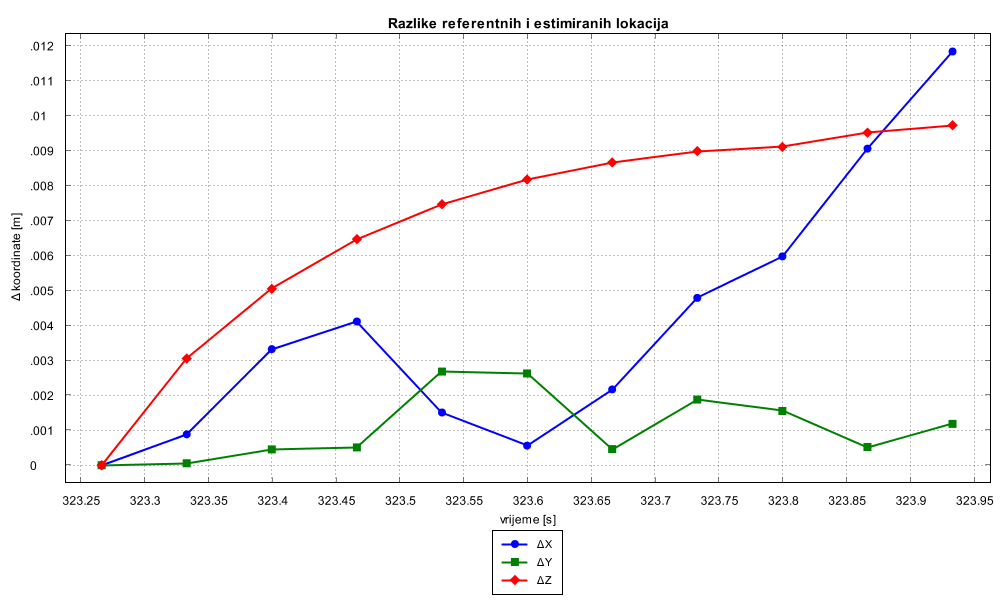
\includegraphics[scale=0.4]{images/imgs/g1_lokacije.png}
  \caption{Primjer 5 - Graf usporedbe lokacija vozila}
  \label{eval:primjer_5_rotacija}
\end{figure}
\begin{figure}[H]
  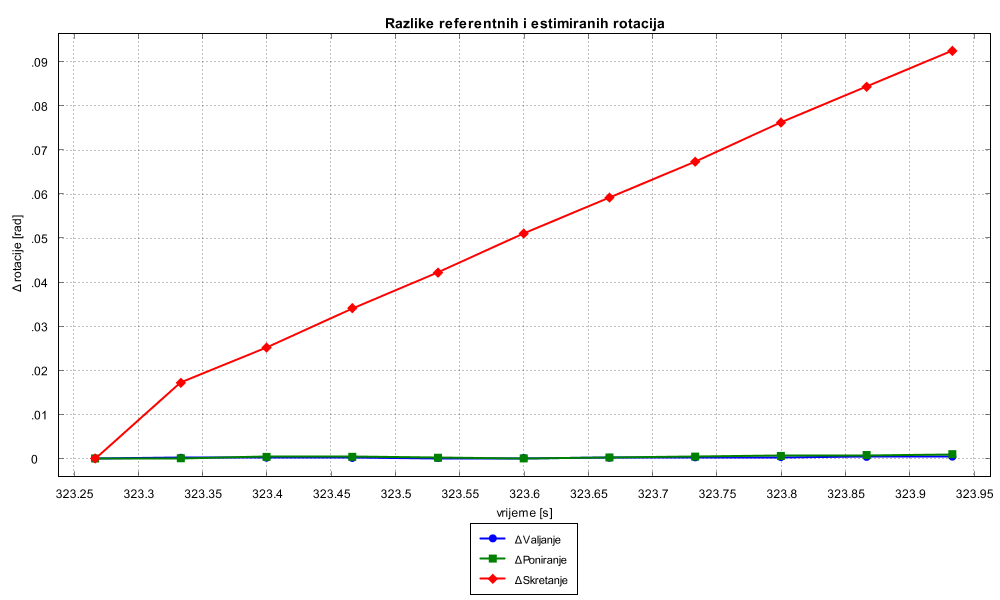
\includegraphics[scale=0.4]{images/imgs/g1_rotacije.png}
  \caption{Primjer 5 - Graf usporedbe rotacija vozila}
  \label{eval:primjer_5_rotacija}
\end{figure}
\begin{figure}[H]
  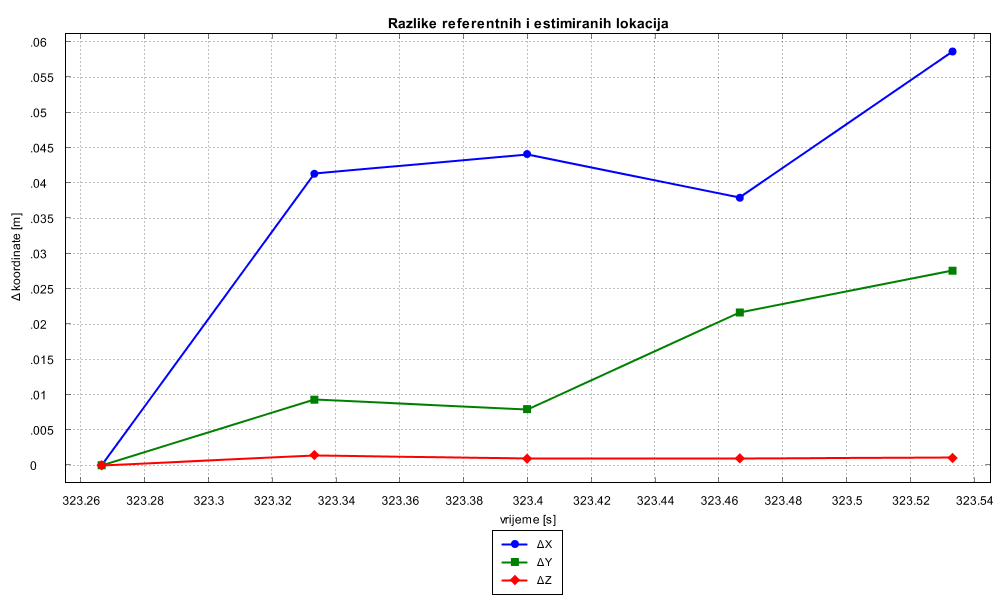
\includegraphics[scale=0.4]{images/imgs/g2_lokacije.png}
  \caption{Primjer 6 - Graf usporedbe lokacija vozila}
  \label{eval:primjer_6_rotacija}
\end{figure}
\begin{figure}[H]
  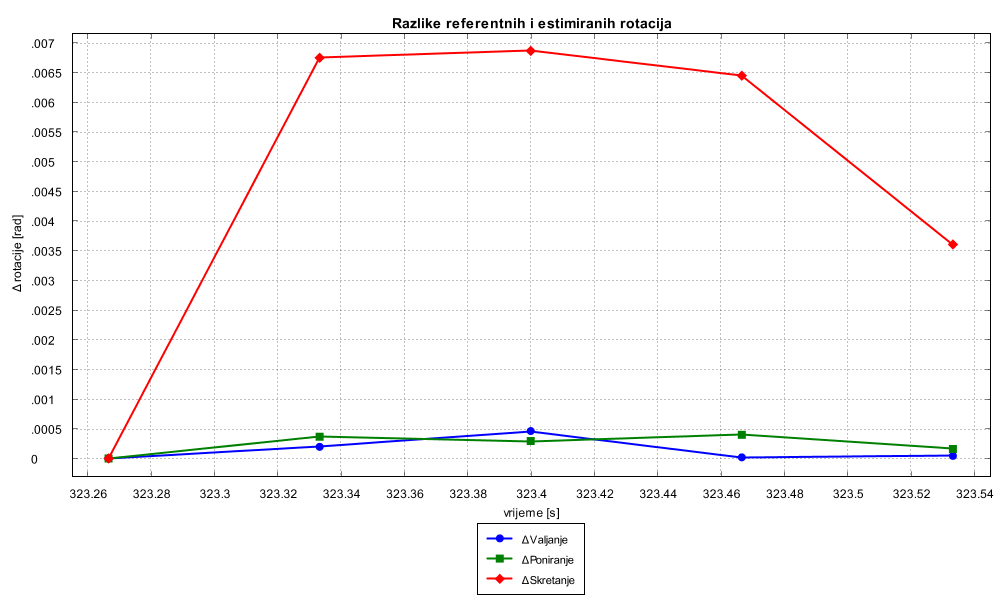
\includegraphics[scale=0.4]{images/imgs/g2_rotacije.png}
  \caption{Primjer 6 - Graf usporedbe rotacija vozila}
  \label{eval:primjer_6_rotacija}
\end{figure}
\pagebreak
\section{ICP algoritam s grupiranjem točaka}
Eksperimantalni rezultati za ICP algoritam s grupiranjem točaka su prikazani u sljedećim tablicama i grafovima. Grafovi i tablice se odnose na podskupove točaka primjera A i B. Uspoređivanjem tablica i grafova može se vidjeti da ICP algoritam s grupiranjem točaka uglavnom bolje estimira rotacije, a nekada i lokacije naspram običnoga generalizirajućeg ICP algoritma.

\subsubsection{Tablica eksprimentalnih rezultata}
\begin{table}[H]
  \begin{tabular}{ |p{3cm}| |p{2cm}|p{2cm}|p{2cm}|p{2cm}| }
    \hline
    Rezultati& Primjer 1& Primjer 2&Primjer 3& Primjer 4\\
    \hline
    AMx [$m$]& 0.18283& 1.294772& 4.58685E-4& 0.18752\\
    AMy [$m$]& 15.2912& 6.7612E-3& 3.4089E-4& 16.36098\\
    AMz [$m$]& 2.06568E-2& 3.42104E-3& 1.18857E-3& 0.017125\\
    AMr [$rad$]& 1.25836E-3& 2.11339E-4& 8.59544E-5& 1.14017E-3\\
    AMp [$rad$]& 2.94473E-3& 2.86964E-4& 4.90207E-5& 3.60941E-3\\
    AMy [$rad$]& 6972636& 2.5872& 2.614223e*4& 6.90612E-3\\
    \hline
    MSEx [$m^2$]& 3.94724E-2& 4.90112& 4.20784E-7& 4.09558E-2\\
    MSEy [$m^2$]& 330.869234& 6.24971E-5& 2.32425E-7& 367.24570\\
    MSEz [$m^2$]& 6.77314E-4& 4.62250E-5& 2.82541E-6& 3.46930E-4\\
    MSEr [$rad^2$]& 1.39011E-5& 6.25045E-8& 1.477634-8& 1.25063E-5\\
    MSEp [$rad^2$]& 2.64382E-5& 1.29621E-7& 4.80606E-9& 3.19971E-5\\
    MSEy [$rad^2$]& 1.63954E-4& 16.25243& 1.36683E-7& 1.56561E-4\\
    \hline
  \end{tabular}
  \caption{Usporedbe referentnih i estimiranih podataka}
  \label{res:ref_est_table}
\end{table}
\pagebreak
\subsubsection{Grafovi eksprimentalnih rezultata}
\begin{figure}[H]
  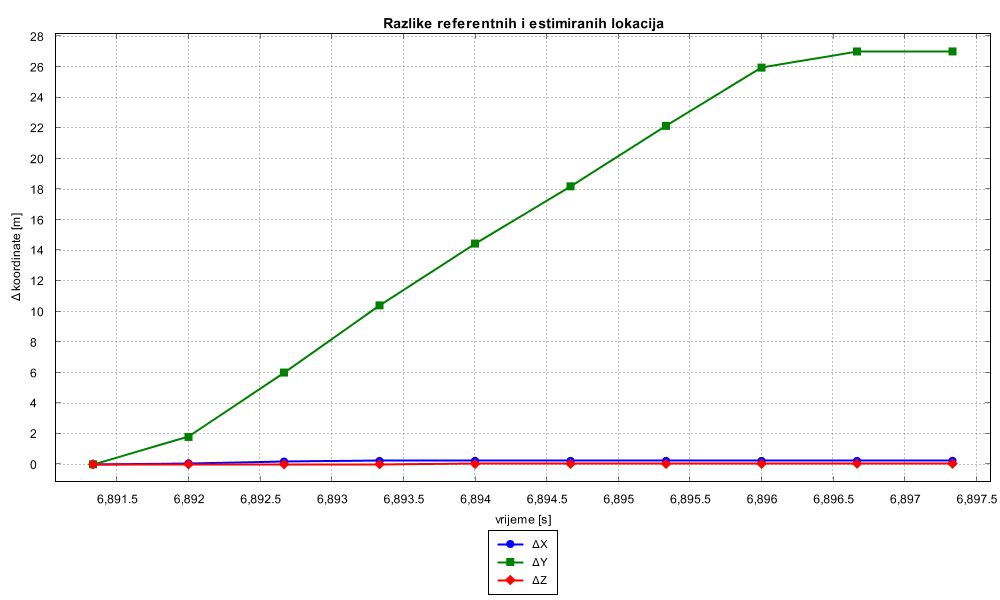
\includegraphics[scale=0.4]{images/imgsvox/1_zavoj_lokacije.png}
  \caption{Primjer 1 - Graf usporedbe lokacija vozila}
  \label{eval:primjer_1_lokacija_vox}
\end{figure}
\begin{figure}[H]
  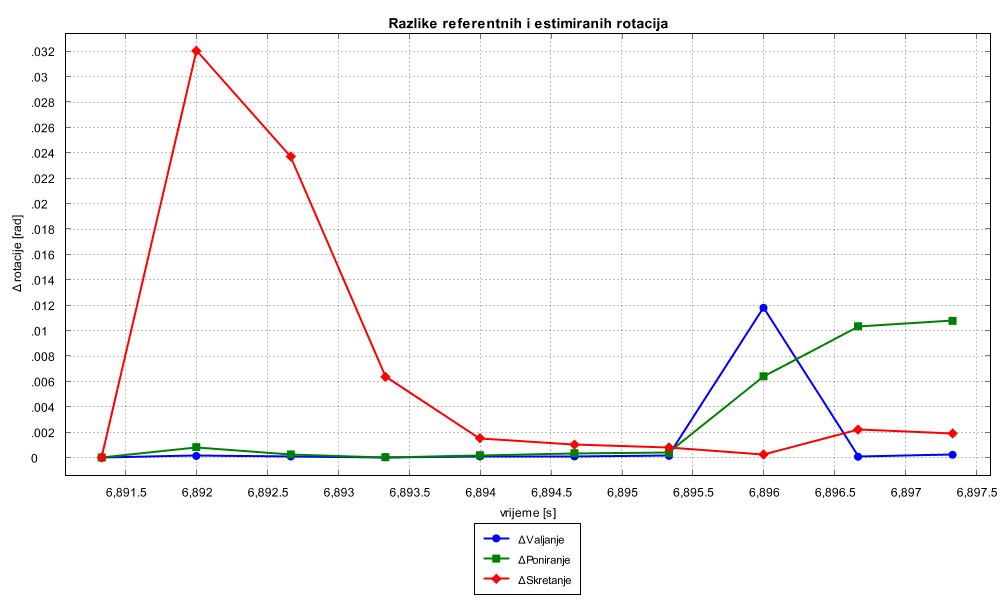
\includegraphics[scale=0.4]{images/imgsvox/1_zavoj_rotacije.png}
  \caption{Primjer 1 - Graf usporedbe rotacija vozila}
  \label{eval:primjer_1_rotacija_vox}
\end{figure}
\begin{figure}[H]
  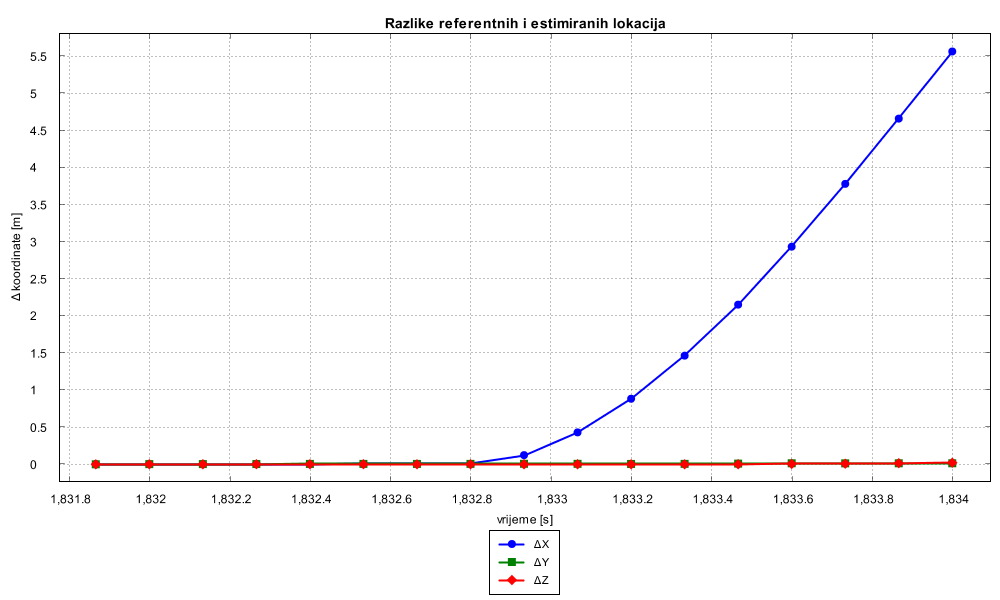
\includegraphics[scale=0.4]{images/imgsvox/2_ravno_lokacije.png}
  \caption{Primjer 2 - Graf usporedbe lokacija vozila}
  \label{eval:primjer_2_lokacija_vox}
\end{figure}
\begin{figure}[H]
  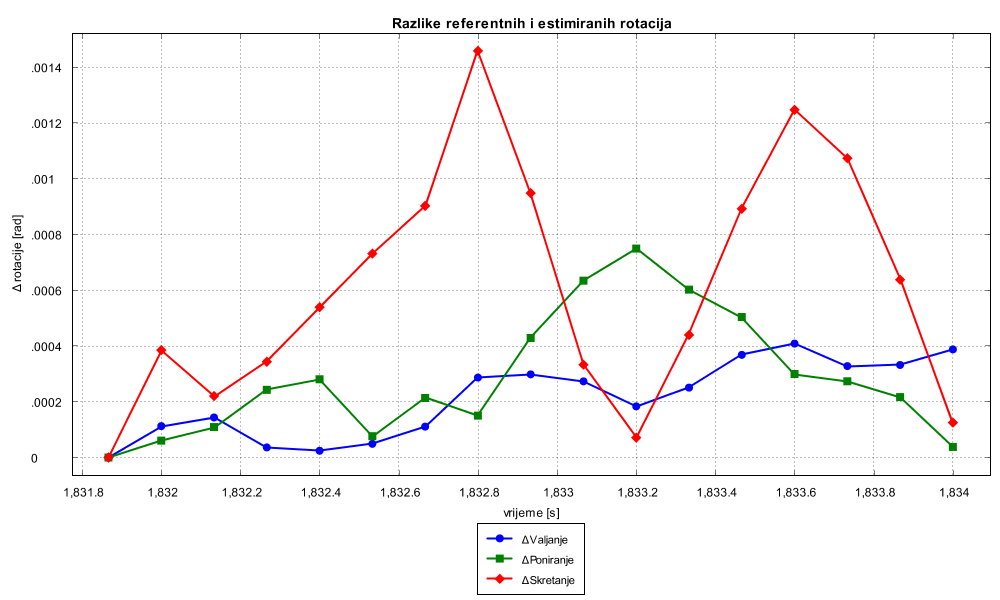
\includegraphics[scale=0.4]{images/imgsvox/2_ravno_rotacije.png}
  \caption{Primjer 2 - Graf usporedbe rotacija vozila}
  \label{eval:primjer_2_rotacija_vox}
\end{figure}
\begin{figure}[H]
  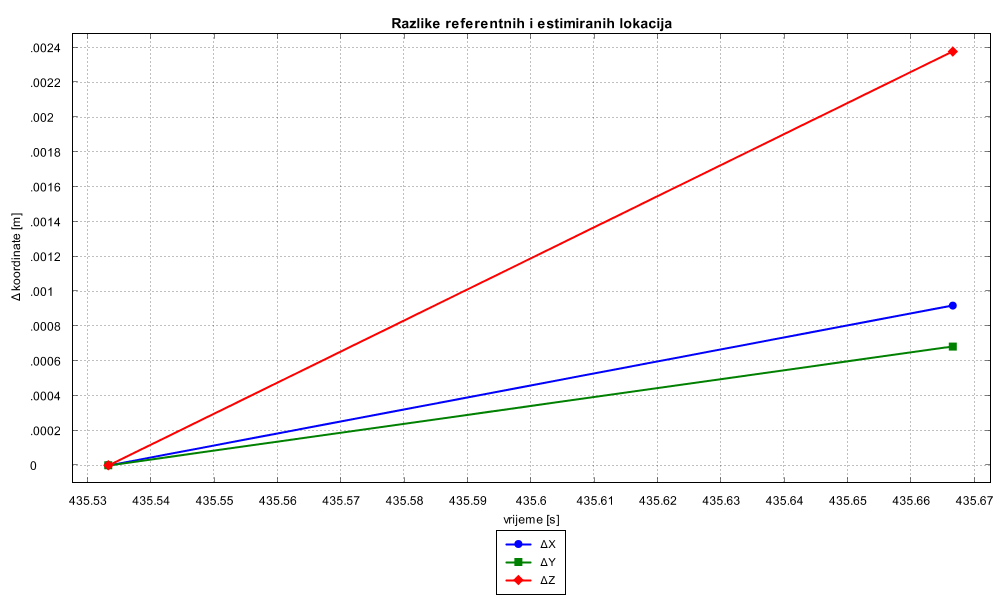
\includegraphics[scale=0.4]{images/imgsvox/3_ravno_lokacije.png}
  \caption{Primjer 3 - Graf usporedbe lokacija vozila}
  \label{eval:primjer_3_rotacija_vox}
\end{figure}
\begin{figure}[H]
  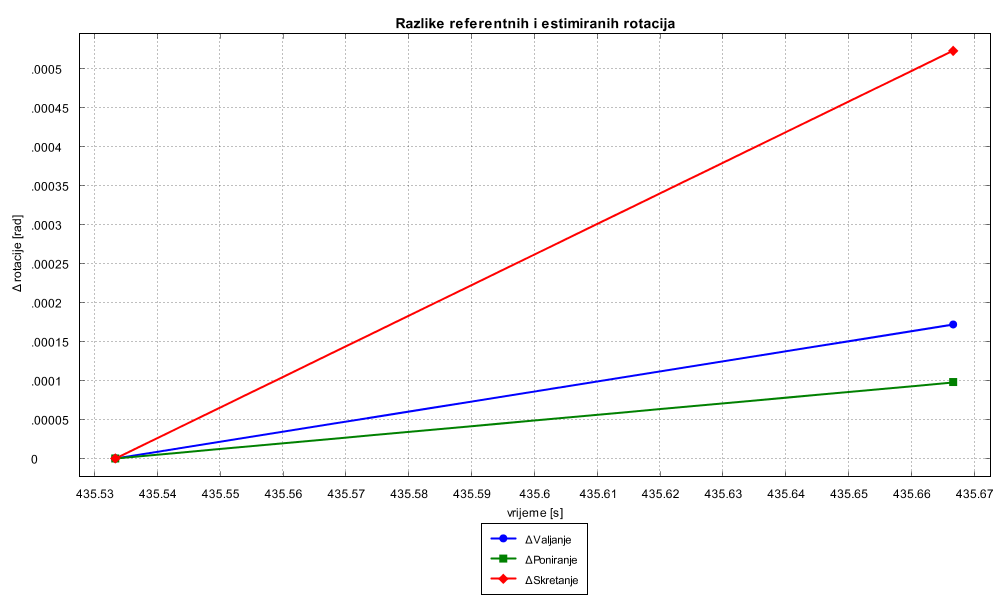
\includegraphics[scale=0.4]{images/imgsvox/3_ravno_rotacije.png}
  \caption{Primjer 3 - Graf usporedbe rotacija vozila}
  \label{eval:primjer_3_rotacija_vox}
\end{figure}
\begin{figure}[H]
  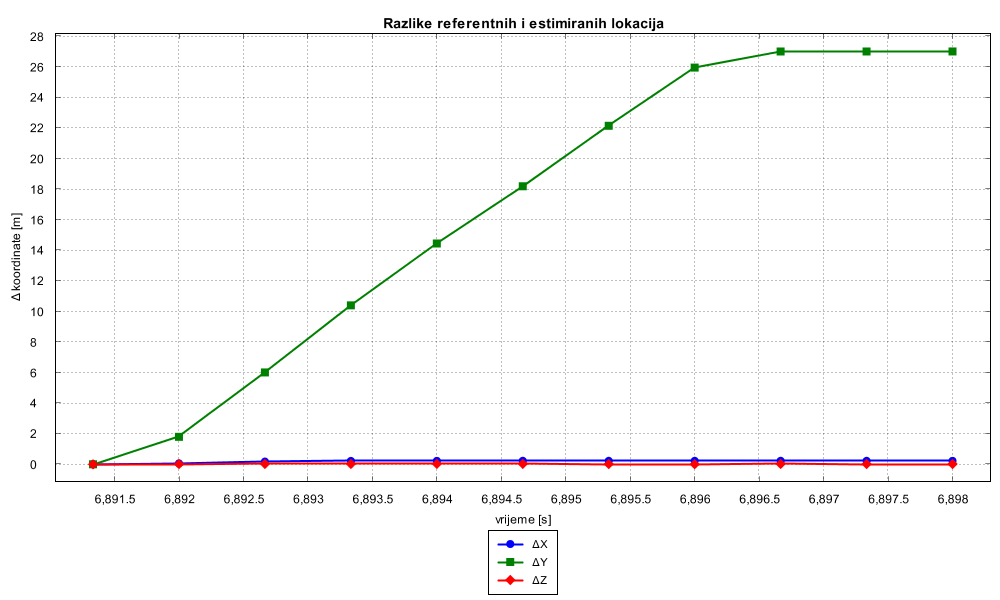
\includegraphics[scale=0.4]{images/imgsvox/4_zavoj_lokacije.png}
  \caption{Primjer 4 - Graf usporedbe lokacija vozila}
  \label{eval:primjer_4_rotacija_vox}
\end{figure}
\begin{figure}[H]
  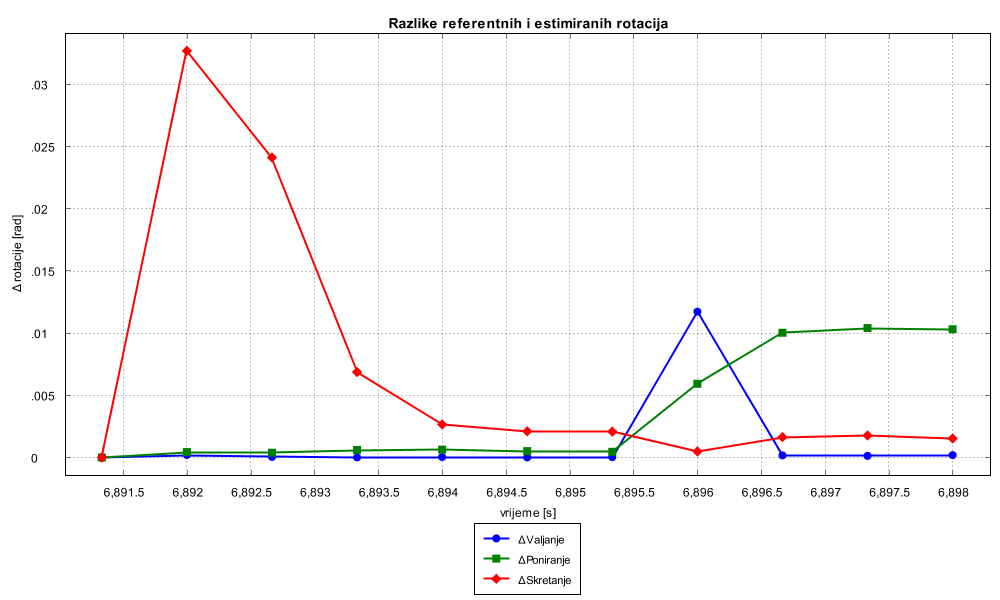
\includegraphics[scale=0.4]{images/imgsvox/4_zavoj_rotacije.png}
  \caption{Primjer 4 - Graf usporedbe rotacija vozila}
  \label{eval:primjer_4_rotacija_vox}
\end{figure}